\graphicspath{ {lecture2/} }
\section{Models of Computation}

What is an Algorithm ? 
\begin{enumerate}
    \item Mathematical abstraction of computer program
    \item Computational procedure to solve a problem
\end{enumerate}

\begin{figure}[H]
    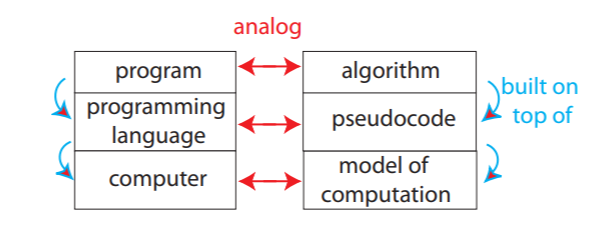
\includegraphics[width=\textwidth]{Figure1}
    \centering
    \caption{Algorithm}
    \label{fig:img1}
\end{figure}


\noindent Model of computation specifies
\begin{enumerate}
    \item what operations an algorithm is allowed
    \item cost (time, space, . . .) of each operation
    \item cost of algorithm = sum of operation costs
\end{enumerate}